% VUT FIT MITAI
% MSZ 2021/2022
% Author: Vladimir Dusek
% Login: xdusek27

%%%%%%%%%%%%%%%%%%%%%%%%%%%%%%%%%%%%%%%%%%%%%%%%%%%%%%%%%%%%%%%%%%%%%%%%%%%%%%%%

\chapter{Správa klíčů v asymetrické kryptografii (certifikáty X.509).}

%%%%%%%%%%%%%%%%%%%%%%%%%%%%%%%%%%%%%%%%%%%%%%%%%%%%%%%%%%%%%%%%%%%%%%%%%%%%%%%%

\section{Metadata}

\begin{compactitem}
    \item Předmět: Kryptografie (KRY)
    \item Přednáška:
    \begin{compactitem}
        \item \path{KRY04_Asym_MNG.pdf}
    \end{compactitem}
    \item Záznam:
    \begin{compactitem}
        \item 2021-03-29
        \item 2021-04-12
    \end{compactitem}
\end{compactitem}

%%%%%%%%%%%%%%%%%%%%%%%%%%%%%%%%%%%%%%%%%%%%%%%%%%%%%%%%%%%%%%%%%%%%%%%%%%%%%%%%

\section{Úvod a kontext}

\textit{Viz. \uv{Úvod a kontext} v předchozích otázkách z tohoto předmětu.}

%%%%%%%%%%%%%%%%%%%%%%%%%%%%%%%%%%%%%%%%%%%%%%%%%%%%%%%%%%%%%%%%%%%%%%%%%%%%%%%%

\section{Správa klíčů v asymetrické kryptografii}

\paragraph*{Problém se zveřejňováním veřejných klíčů} Jak můžu vědět, že publikovaný veřejný klíč patří opravdu entitě, které patřit má? Je potřeba zajistit autenticitu (pravost) veřejných klíčů~--~Vytvořit spolehlivou vazbu mezi veřejným klíčem a jménem jeho vlastníka.

\paragraph*{Certifikát} Certifikace veřejného klíče. Nějaký prostředník (certifikační autorita), kterému důvěřujeme, se zaručuje, že konkrétní veřejný klíč, patří dané entitě.

\paragraph*{Certifikační autorita} Certifikační autorita (CA) je prostředník, který distribuuje certifikáty a které všichni důvěřují.

\paragraph*{Proces certifikace klíče} CA podepíše veřejný klíč uživatele a jeho další údaje (jméno, doba vydání, doba platnosti, \dots) svým vlastním soukromým klíčem. Tyto podepsané údaje se nazývají certifikát.

\begin{figure}[H]
    \centering
    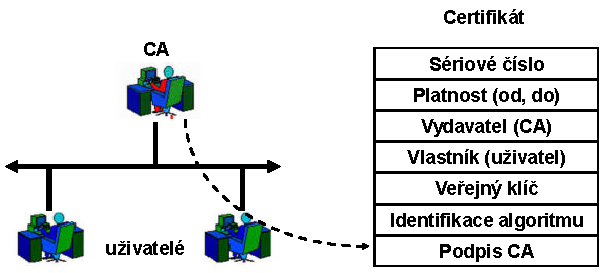
\includegraphics[width=0.65\linewidth]{kry_4/certifikat.pdf}
    \caption{Příklad certifikátu a informací co obsahuje.}
\end{figure}

\begin{figure}[H]
    \centering
    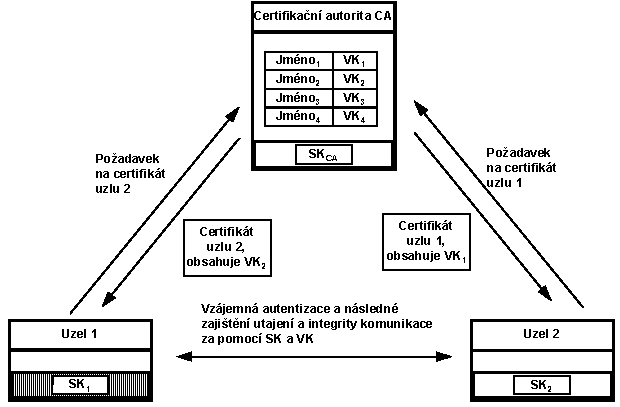
\includegraphics[width=1\linewidth]{kry_4/vymena_certifikatu.pdf}
    \caption{Příklad navázání bezpečné komunikace mezi dvěma entitami, které mají stejnou certifikační autoritu.}
    \label{53_vymena_certifikatu}
\end{figure}

\paragraph*{Navázání bezpečné komunikace} Popis navázání bezpečné komunikace (viz obrázek~\ref{53_vymena_certifikatu}):
\begin{compactenum}
    \item Mějme situaci, kdy strana $A$ odešle straně $B$ digitálně podepsaný soubor. Jak strana $B$ podpis ověří? Nejprve se oveří podpis certifikátu pomocí veřejného klíče příslušné certifikační autority. Poté se ověří podpis dokumentu pomocí veřejného klíče protistrany (ten se nachází v certifikátu). Jediný čemu příjemce musí věřit je veřejný klíč certifikační autority.
\end{compactenum}

\paragraph*{CRL} todo

Strom certifikačních autorit

Kořenová certifikační autorita

Certifikační cesta

Křížový certifikát

\todo{todo}

%%%%%%%%%%%%%%%%%%%%%%%%%%%%%%%%%%%%%%%%%%%%%%%%%%%%%%%%%%%%%%%%%%%%%%%%%%%%%%%%

\section{Standard X.509}

\paragraph*{X.509} X.509 je standard pro systémy založené na veřejném klíči (PKI, \textit{public key infrastructure}). Specifikuje formát certifikátů, seznamy zneplatněných certifikátů (CRL, \textit{anglicky certificate revocation list}), parametry certifikátů, metody kontroly platností certifikátů, \dots
